\section{State of the Art} \label{sec:sota}
This section will discuss the existing smart materials that are currently studied and used in the domain of actuators. The different techniques and integration systems will also be presented with the goal to compare the various approaches currently used.

\subsection{Smart materials} \label{subsec:Smartmaterials}
In the field of engineering, ranging from haptics, automation and bio-medical fields, there has been a need  to create actuators that are lightweight, compact and having force output. This creates a need for materials that can deliver high forces and strokes while remaining light and small meaning that the materials need to have a high work output.

On the basis of creating an actuator that can meet the demands of the currently implemented strategies while at the same time pushing the limits of the current technology, a thorough investigation of the available smart materials must be conducted. These materials have the ability to react to an external stimulus such as thermal electrical or magnetic and are thus referred to as \emph{smart} or \emph{active materials}. These materials have an inherent property that allows them to be exploited with a specific external stimulus so as to alter their mechanical characteristics or to create self-sensing technology.

There exist numerous types of smart materials and based on their properties, they can be classified into many types such as \cite{damodharan_review_2018}:
\begin{itemize}
	\item Piezoelectric materials
	\item Magneto-strictive materials
	\item Electro-active polymers
	\item Shape Memory Alloys
\end{itemize}

The aim of this project is to adapt these aforementioned smart materials to harness their specific behaviour and fabricate smart actuators. This implies that the system that incorporates the material is equally critical for the conception of the actuator. This section of the report will delved into different strategies used to harness the specific behaviours of the smart materials and integrate them into actuators.

\subsubsection{Piezoelectric Materials}
Piezoelectric materials are a subgroup of smart materials that have the capability to produce voltages when a stress is applied. This behaviour is can also be expressed in the opposite direction i.e. a strain can be generated using an electric field. Piezoelectric materials are the most popular type of smart materials and the most commonly used piezoceramics, such as lead zirconate titanate, are available in the form of thin sheets. These sheets can then be stacked to create piezostack actuators.

\subsubsection{Magneto-strictive materials}
The magneto-strictive materials are category of smart materials that have the ability to alter their mechanical behaviour and shape when subjected to magnetic fields. Magnetic Shape Memory Alloys (MSMA) are a popular type of magnet0-strictive material. Here, the MSMA shows an interesting behaviour in which the material when deformed will tend to remain stable and retain its deformed shape. As the materials is introduced into a strong magnetic field, the crystals of the material are realigned and the material reverts back to its predeformed shape.

\subsubsection{Electro-Active polymers}

\subsubsection{Shape Memory Alloys}
Shape Memory Alloys (SMA) are a particular subgroup of smart materials that change their mechanical behaviour based on a thermal stimulus. Here, the material as with the MSMA, retains its shape when deformed and reverts back to its original shape when heated. Shape Memory Alloys (SMA) actuators provide us with an opportunity to create such actuators due to their high work output per volume which is around 10 $\mathrm{J}/\mathrm{cm}^3$\cite{MohdJani2014}. This can be a 10-fold increase when compared to pneumatic actuators. The SMA actuators are thus able to provide large amounts of force when compared to their volume, making them particularly useful in compact, lightweight actuators.

NiTiNOL, the most used SMA, contains an interesting property known as the Shape Memory Effect (SME), which allows the material to return to its unloaded state when it is heated above its transition temperature.

Shape memory alloys such NiTiNOL show two important properties: the Shape Memory Effect (SME) and Superelasticity (SE)\cite{Rao2015}. The property, this device aims to exploit is the SME. Materials exhibitng this property are able to return to a pre-defined shape when heated through a certain temperature range.

SMAs exist in various different stable phases which consists of the \emph{Martensitic (M)} phase and the \emph{Austenitic (A)} phase. The M phase can exist in either the \emph{Twinned M phase} or the \emph{Detwinned M phase} based on the stress experienced by the material. The SME is the effect that transforms the material from the A phase to its M phase, also known as the Martensitic transformation. The opposite transformation, from the M phase to the A phase, is known as Austenitic transformation. When the material reaches the Austentic transformation temperature ($\mathbf{A_s}$) threshold, the material will begin the Austenitic transformation. Inversely, as the material cools down to the Martensitic transformation temperature ($\mathbf{M_s}$), it will begin the Martensitic transformation. Since these transformations occur over a range in temperature, we must heat and cool well beyond the transformation temperatures.

The buckled SMA beam will make use of an SMA with a relatively high transformation temperature (with $A_s$ around 50\degreeC) and thus exists primarily in the M phase at room temperature. The phase transformations can be seen in figure \ref{fig:PhaseTransfDiagram}. When a mechanical load is applied to the SMA while in its M phase, the material shears on an atomic level and this allows it to deform through a detwinning process at relatively low stress levels. This process allows the material to deform up to strains of 8$\%$. Strains larger than this will cause dislocations which are irreversible. When the beam is then heated, the Austentite transformation from the detwinned M phase to the A phase, causes the beam to lose all the strain due to twinning, allowing the material to return to its original shape. This strain recovery allows the beam to revert to its pre-defined state while producing large forces.

\begin{figure}[H]
  \centering
  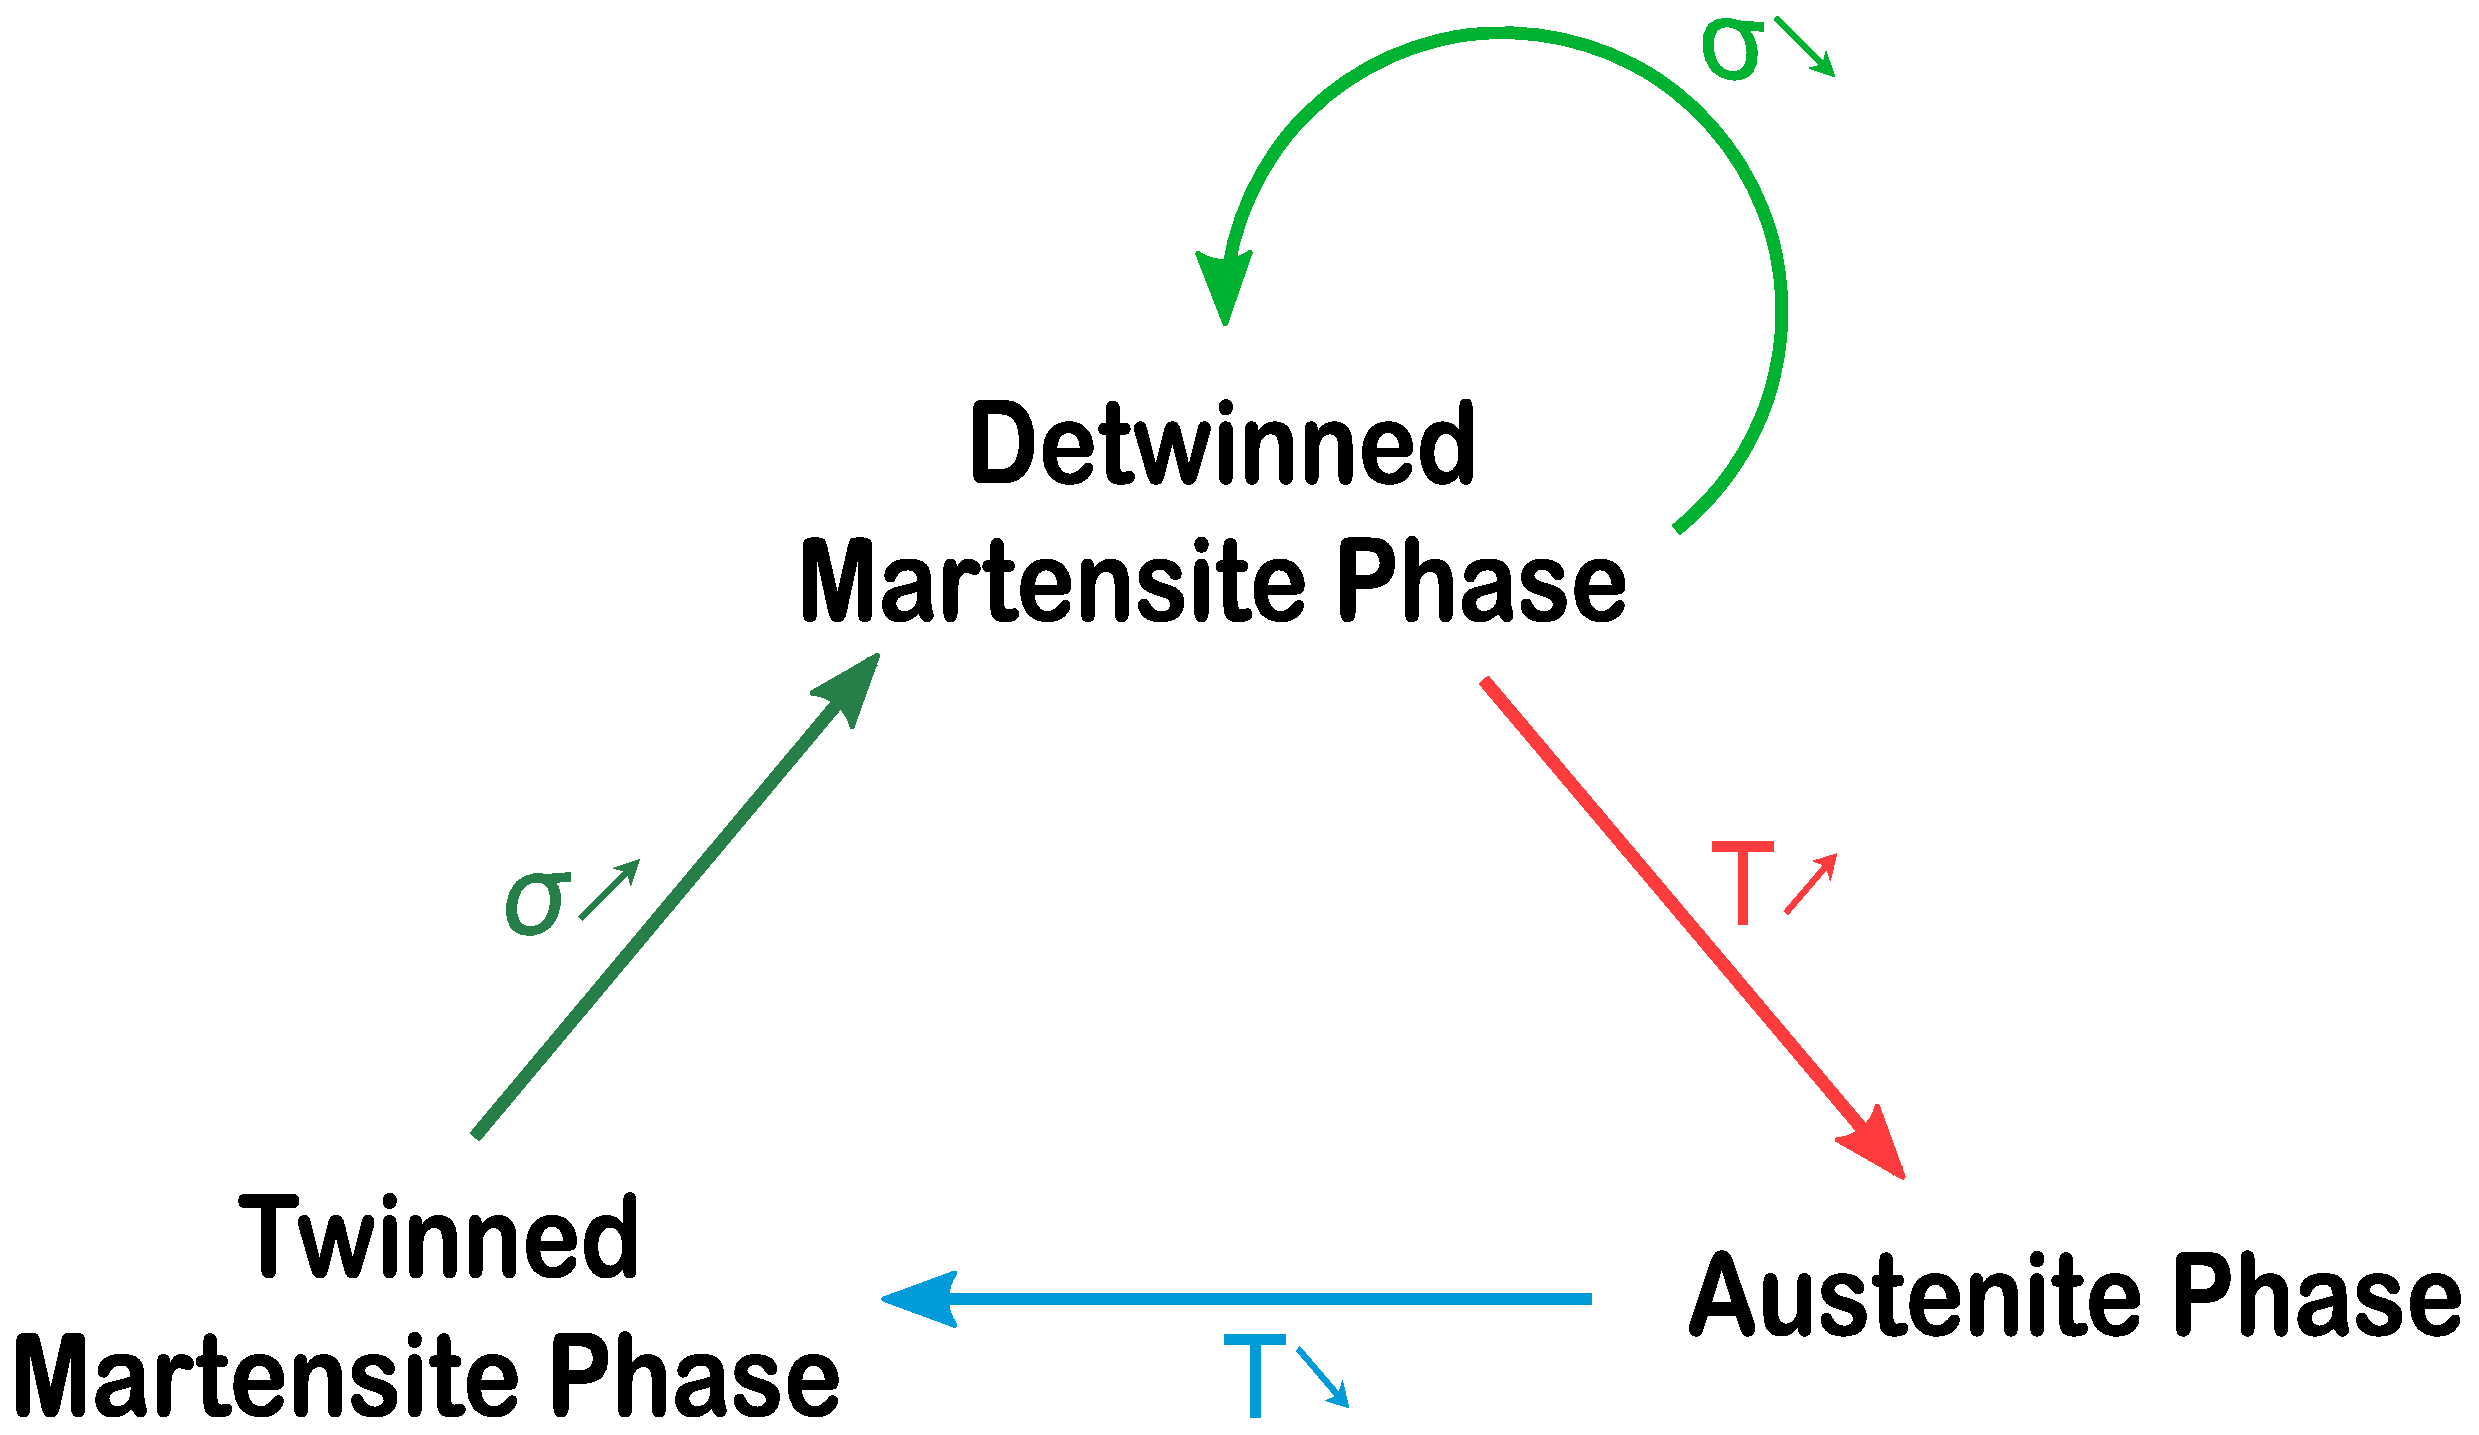
\includegraphics[width=0.5\textwidth]{Figures/Phase_Transf_Diagram_noText.eps}
  \caption{Phase transformation diagram of a shape memory alloy. Here $\sigma$ represents the stress created by mechanical loading and T represents the temperature change due to thermal loading.}
  \label{fig:PhaseTransfDiagram}
\end{figure}
